\documentclass[fleqn,10pt,twoside]{gcb15submission}
\usepackage{url}\urlstyle{same}
\usepackage{booktabs}
\usepackage{colortbl, xcolor}
\usepackage{tabularx}
\usepackage{multirow}
\usepackage{epstopdf}

\newcommand*{\bigcdot}{\raisebox{-0.25ex}{\scalebox{1.5}{$\cdot$}}}


\title{Prediction of amyloidogenicity based on the n-gram analysis}


\author[1]{Micha\l{} Burdukiewicz}
\author[2]{Piotr Sobczyk}
\author[3]{Stefan R\"{o}diger}
\author[4]{Anna Duda-Madej}
\author[1]{Pawe\l{} Mackiewicz}
\author[5]{Ma\l{}gorzata Kotulska}
\affil[1]{University of Wroc\l{}aw, Department of Genomics}
\affil[2]{Wroc\l{}aw University of Science and Technology, Faculty of Pure and Applied Mathematics}
\affil[3]{Brandenburg University of Technology Cottbus-Senftenberg, Institute of Biotechnology}
\affil[4]{Wroclaw Medical University, Department of Microbiology}
\affil[5]{Wroc\l{}aw University of Science and Technology, Department of Biomedical 
Engineering, Faculty of Fundamental Problems of Technology}

\keywords{n-gram, amyloid, prediction, random forest, feature selection}

\begin{abstract}
Amyloids are proteins associated with the number of clinical disorders (e.g., Alzheimer's, Creutzfeldt-Jakob's and Huntington's diseases). Despite their diversity, all amyloid proteins can undergo aggregation initiated by 6- to \mbox{15-residue} segments called hot spots. To find the patterns defining the hot-spots, we trained predictors of amyloidogenicity based on random forests using short subsequences (n-grams) extracted from amyloidogenic and non-amyloidogenic peptides collected in the AmyLoad database. Since the amyloidogenicity may not depend on the exact sequence of amino acids but on more general properties of amino acids, we tested 524,284 reduced amino acid alphabets of different lengths (three to six letters) to find an alphabet providing the best performance of the predictor in cross-validation. The predictor based on this alphabet, called AmyloGram, was benchmarked against the most popular tools for the detection of amyloid peptides using an external data set and obtained the highest values of performance measures (AUC: 0.90, MCC: 0.63). Additionally, our results showed that the amyloidogenicity is strongly correlated with hydrophobicity, a tendency to form $\beta$-sheets and rigidity of amino acid residues. After the reduction of amino acids in peptides using the best-performing alphabet, among the most informative n-grams we identified 15 that were already confirmed experimentally. 
AmyloGram is available as a web-server: \url{www.smorfland.uni.wroc.pl/amylogram/}. The code and results are publicly available at: \url{github.com/michbur/prediction_amyloidogenicity_ngram}.

\end{abstract}


\begin{document}


\flushbottom
\maketitle
\thispagestyle{empty}



\section{Introduction}

Amyloid aggregates have been observed in tissues of people suffering from 
various diseases, such as: Alzheimer's, Parkinson's, Huntington's and 
amyotrophic lateral sclerosis, as well as many other 
conditions~\citep{vidal_characterization_2011}. These aggregates were also 
detected in disorders other than neurological, for example in diabetes of type 2 
or certain types of a cataract. Cells in tissues with amyloid oligomers exhibit 
very high mortality. However, the exact mechanisms of the cytotoxicity have not 
been discovered. The aggregates are very stable and their dissolution is very 
difficult. Amyloids are resistant to activity of proteolytic enzymes and 
chemical compounds due to the specific and highly ordered structure of their 
steric zipper. However, some strategies to prevent amyloid formation have been 
proposed, e.g. ~\citet{hard_inhibition_2012}.

  The aggregation occurs when a cell environment fosters the partial unfolding 
of protein chains or their fragmentation in such a way that the parts prone to 
joining with similar protein fragments become exposed. 
%For the majority of 
%proteins, considerable conformational rearrangement must have occurred to 
%initiate the aggregation process. Such changes cannot take place in the 
%typical 
%tightly packed native protein conformation due to the constraints on the 
%tertiary structure. T
The formation of the non-native partially unfolded 
conformation is required to start the aggregation, presumably by enabling 
specific intermolecular interactions including electrostatic attraction, 
hydrogen bonding and hydrophobic contacts~\citep{chaturvedi_protein_2016}. 
%This 
%partial unfolding can be 
%influenced by various factors, such as high concentration of proteins, high 
%temperature, low pH, binding metals, or exposition to UV 
%light.

  Initially, the resulting molecules form clusters consisting of a few elements, 
which are called oligomers. Next, they grow into larger aggregates. The 
aggregation of proteins or their fragments may lead to amorphous (unstructured) 
clusters or amyloid (highly ordered) unbranched fibrils. Independently of the 
protein sequence and its original structure, aggregates always display a common 
cross-$\beta$ structure~\citep{sawaya_atomic_2007}. The distinctive structure of 
the steric zipper enables the selective detection of amyloids from amorphous 
aggregates using either a variety of microscopic techniques or fluorescence of 
probes with which they form compounds.

  Currently, it is believed that short peptide sequences of amyloidogenic 
properties, called hot spots, are responsible for the aggregation of amyloid 
proteins. Previous studies have suggested that amyloidogenic fragments may have 
regular characteristics, not only with regard to averaged physicochemical 
properties of their amino acids, but also the order of amino acids in the 
sequence. 

  It is important to distinguish between amyloidogenic and amyloid (or 
amyloidic) peptides, because only the former are capable of initiating the 
process of aggregation. The latter may consist of amyloidogenic hot-spots as 
well as other regions that are not directly responsible for the onset of 
aggregation process, although involved in the final aggregate. Several 
computational approaches have been proposed to model and predict both kinds of 
regions. Physics- and chemistry-based models used in  
FoldAmyloid~\citep{garbuzynskiy_foldamyloid:_2010} and 
PASTA2~\citep{walsh_pasta_2014} utilize the density of the 
protein contact sites. 
%Other methods perform threading a peptide on an amyloid 
%fiber backbone, followed by determination of its energy and 
%stability~\citep{odonnell_method_2011}. 
Statistical approaches include production of frequency profiles, such as the 
WALTZ method 
\citep{maurer-stroh_exploring_2010} and machine learning methods, for example 
those 
developed in our group \citep{stanislawski_machine_2013, gasior_fish_2014} and
novel predictor based on neural networks~\citep{familia_prediction_2015}. 
%AGGRESCAN3D was proposed to estimate more accurately aggregation propensity by 
%performing 3D structure based analysis~\citep{zambrano_aggrescan3d_2015}. 


% * <kotulska@gmail.com> 2016-06-12T07:45:50.734Z:
%
% >   The majority of methods described above uses theoretical knowledge to 
% > specify decision rules determining the presence of the hot spot
%
% Z tym się nie zgadzam bo wzorce czestotliwosciowe (Waltz) albo uczenie maszynowe tego nie robią. Jakoś nie bardzo czuję znaczenie tego akapitu. Może jakoś "accepts the whole set of decission rules generated by the method"
%
% ^.
  The aim of our study is to choose out of thousands of created hot spot 
models the most appropriate one and from its analysis gain a new insight into the 
mechanism of amyloidogenicity. To do so, we combined n-gram analysis with the
reduction of amino acid alphabet.
  
  In bioinformatics, n-grams (k-mers) are continuous or discontinuous sequences 
of $n$ elements. Employed as a feature extraction method, n-grams are widely 
used in various analyses of biological sequences. Our choice of n-grams was driven by 
their highly interpretable nature. This is a valuable feature because we are 
interested in identification of motifs that are most relevant to amyloidogenic 
properties of peptides.

  Several studies highlighted that three-dimensional protein structure depends 
not on the exact sequence of amino acids but also on their general physicochemical 
properties. Hence, the 20-letter amino acid alphabet reduced into a smaller 
alphabet (encoding), which represents certain subgroups of aminoacids, 
can still retain the information about the protein folding~\citep{murphy_simplified_2000}. 
Since amyloid aggregates, especially 
their hot spots regions, have very specific spatial organization, we 
investigated if these regions can be also described by a shorter amino acid 
alphabet. Instead of relying on the general similarities of amino acids, we 
% * <kotulska@gmail.com> 2016-06-12T08:03:04.078Z:
%
% > Since amyloid aggregates, especially 
% > their hot spots regions, have very specific spatial organization, we 
% > investigated if these regions can be also described by a shorter amino acid 
% > alphabet
%
% Usunęłabym to zdanie. Jest powtórzeniem poprzedniego.
%
% ^ <michalburdukiewicz@gmail.com> 2016-06-12T18:07:51.663Z:
%
% zmodyfikowałem to zdanie. Teraz w pierwszym zdaniu wprowadzamy ideę zmniejszania alfabetu przy zachowaniu informacji o foldingu (Hence, the 20-letter amino acid alphabet...), a w następnym ("Since amyloid aggregates, especially... ") jak można to zastosować do amyloid.
%
% ^.
created multiple encodings based on the combinations of various physicochemical 
properties that might be associated with amyloidogenicity.  

  To discover amino acid patterns specific for amyloidogenicity, we based our 
analysis on n-grams, continuous or discontinuous sequences of length $n$ drawn 
from the encoded peptides. The extraction of n-grams allows the detection of 
more elaborated motifs, but creates very large features spaces. Henceforth, we 
used a novel feature selection algorithm, Quick Permutation Test (QuiPT), to 
select the most informative n-grams.

  We used selected n-grams to train a predictor based on the random 
forest method~\citep{breiman_random_2001} to discriminate between amyloidogenic and 
non-amyloidogenic peptides. We trained the classifier for several iterations on 
peptides of varying lengths to identify the optimal number of residues which 
include the information about the occurrence or absence of a hot spot. In the 
cross-validation setup, we found the encoding associated with the best-performing 
classifier and its set of informative n-grams. Finally, we benchmarked our 
best-performing classifier, AmyloGram, on an external data set against 
state-of-art software tools for prediction of amyloid or amyloidogenic regions.

\section{Methods}

\begin{figure*}[bth]
\centerline{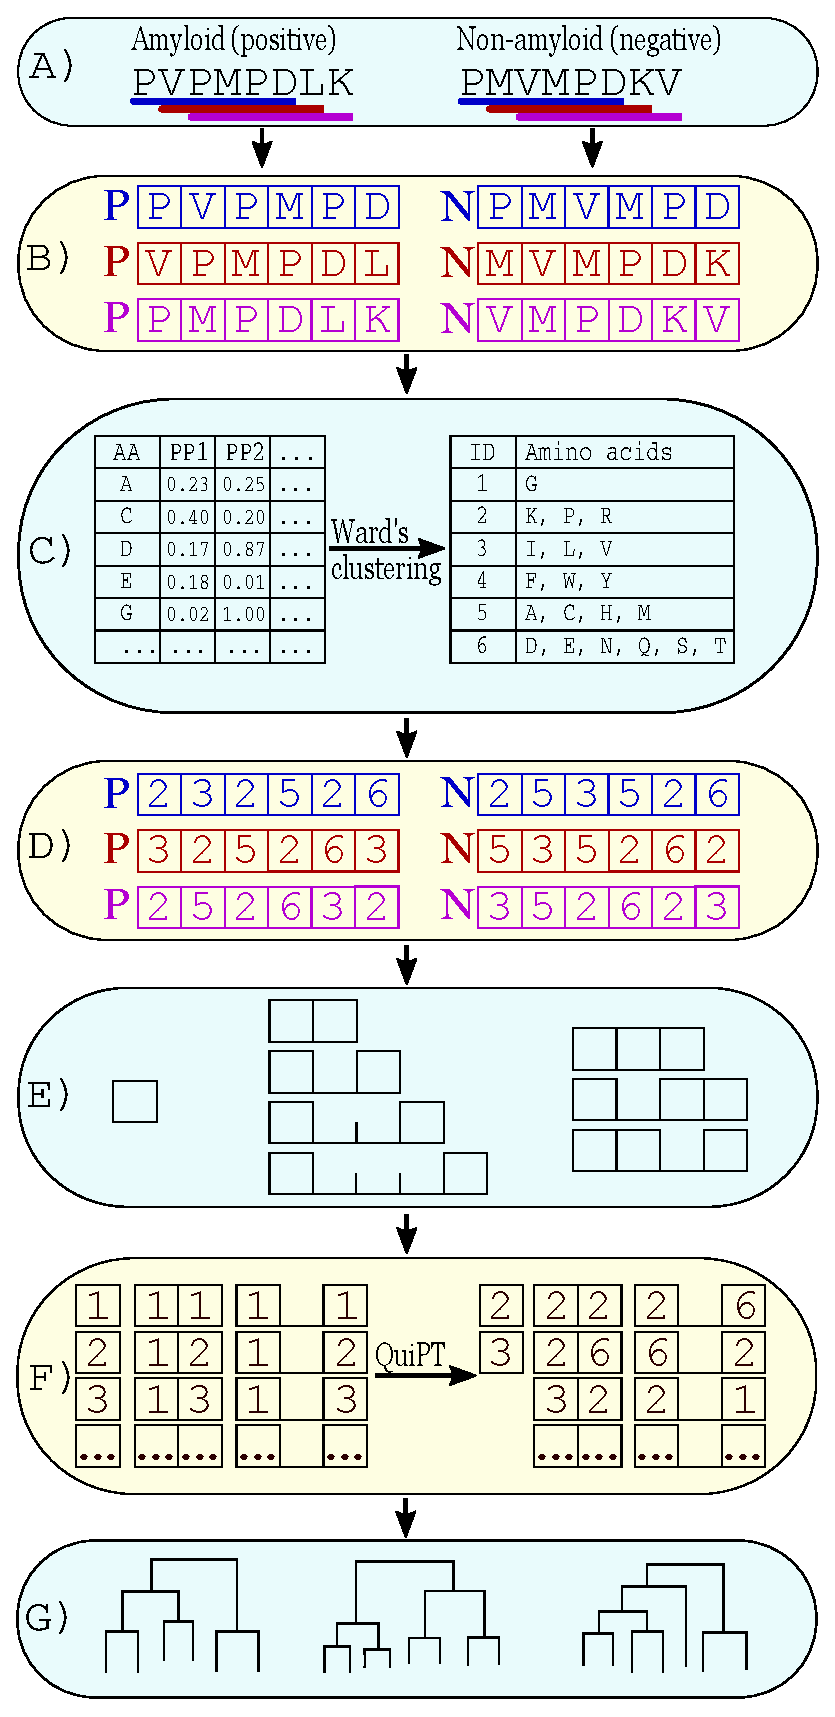
\includegraphics[width=0.3\linewidth]{figures/ngram_scheme.eps}} 
\caption{The scheme of n-gram extraction from studied peptide sequences. 
A) Source data: peptides with known amyloidicity status and indicated 
overlapping hexamers. 
B) Extraction of the overlapping hexamers with ascribed the 
amyloid status taken from their source peptide (P-positive, N - 
negative). 
C) Clusterization of amino acids into an encoding using a combination of 
various 
physicochemical properties (PP). 
D) Reduction of the amino acid alphabet in hexamers. 
E) Extraction of n-grams. From each hexamer, we extracted continuous n-grams 
with the length n = 1, 2 or 3. In addition, we selected gapped 2-grams with a 
gap of the length from 1 to 3 residues and gapped 3-grams with a single gap 
between the first and the second or the second and the third element of the 
n-gram.
F) Selection of informative n-grams with Quick Permutation Test (QuiPT).
G) Training of a random forest classifier using the n-grams selected in the 
previous 
step.}\label{fig:ngram_scheme} 
\end{figure*}

\subsection{Data set}

\begin{table}[h]
\centering
\small
\caption{Characteristics of training and test data sets used in the 
cross-validation. All sequences were derived from AmyLoad database. Training 
data sets are partially overlapping (e.g. $[6, 10]$ contains also sequences 
from $[6, 7)$). Test data sets are always disjointed.}
\label{tab:data_sets}
\begin{tabular}{cccll}
\toprule
Set & Sequence length & Status & Sequences & Hexamers \\ 
\midrule
\multirow{6}{*}{Training} & \multirow{2}{*}{[6-7)} & Non-amyloid & 841 & 841 
\\
 &  & \cellcolor[gray]{0.85}Amyloid & \cellcolor[gray]{0.85}247 & 
\cellcolor[gray]{0.85}247 \\
 \cline{2-5}
 & \multirow{2}{*}{{[}6,10{]}} & Non-amyloid & 964 & 1412 \\
 &  & \cellcolor[gray]{0.85}Amyloid & \cellcolor[gray]{0.85}312 & 
\cellcolor[gray]{0.85}475 \\
 \cline{2-5}
 & \multirow{2}{*}{{[}6,15{]}} & Non-amyloid & 992 & 1653 \\
 &  & \cellcolor[gray]{0.85}Amyloid & \cellcolor[gray]{0.85}342 & 
\cellcolor[gray]{0.85}720 \\
 \hline
 \hline
\multirow{8}{*}{Test} & \multirow{2}{*}{6} & Non-amyloid & 841 & 841 \\
 &  & \cellcolor[gray]{0.85}Amyloid & \cellcolor[gray]{0.85}247 & 
\cellcolor[gray]{0.85}247 \\
 \cline{2-5}
 & \multirow{2}{*}{{[}7,10{]}} & Non-amyloid & 123 & 571 \\
 &  & \cellcolor[gray]{0.85}Amyloid & \cellcolor[gray]{0.85}65 & 
\cellcolor[gray]{0.85}228 \\
 \cline{2-5}
 & \multirow{2}{*}{{[}11,15{]}} & Non-amyloid & 28 & 241 \\
 &  & \cellcolor[gray]{0.85}Amyloid & \cellcolor[gray]{0.85}30 & 
\cellcolor[gray]{0.85}245 \\
 \cline{2-5}
 & \multirow{2}{*}{{[}16,25{]}} & Non-amyloid & 41 & 571 \\
 &  & \cellcolor[gray]{0.85}Amyloid & \cellcolor[gray]{0.85}55 & 
\cellcolor[gray]{0.85}778 \\
 \bottomrule
\end{tabular}
\end{table}

The data used in the study was extracted from AmyLoad data 
base~\citep{wozniak_amyload:_2015}. We obtained 418 amyloidogenic peptides and 
1039 non-amyloidogenic peptides.

  Sequences shorter than six and longer than 25 amino acid residues (i.e., 8 and 
27 sequences, respectively) were removed from the set. The former were too short 
to be processed in the devised n-gram analysis framework and the latter were too 
diversified and rare, hampering the proper analysis.

  The final data set contained in total 1430 peptides: 397 amyloidogenic 
% * <kotulska@gmail.com> 2016-06-12T08:24:11.292Z:
%
% > amyloidogenic
%
% Zastanawiam się czy tu nie napisać " amyloid - zamiast amyloidogenic (podobne w dalszej części zdania). Tak naprawdę to n-gramy są uczone jednak wg. amylodowości a nie hot-spotów - a w swoim celu maja samodzielne wyciągniecie z tego hot-spotów. Co jest przecież ciekawą cechą tej metody. Czy mam rację?
%
% ^ <michalburdukiewicz@gmail.com> 2016-06-12T18:10:00.546Z:
%
% a czy w bazie AmyLoad nie mamy wyłącznie hot spotów? Mam wrażenie, że te peptydy o długości 6-25 aa to jednak wyłącznie hot spoty
%
% ^.
and 1033 non-amyloidogenic (and non-amyloid) sequences. 

\subsection{Encodings of amino acids}

The amyloidogenicity of a given peptide may not depend on the exact sequence of 
amino acids but on their more general properties. To verify this hypothesis, we 
handpicked 20 different measures from AAIndex data base~\citep{kawashima_aaindex:_2008} 
describing features important in the amyloidogenicity, such as: size of 
residues, hydrophobicity, solvent surface area, frequency in $\beta$-sheets and 
contactivity. We preferred more accurate measures introduced after 1980. 
The set of selected physicochemical properties was enriched by 
six measures representing amino acid contact site 
propensities~\cite{wozniak_characteristics_2014}. This gave us  26 features in total .

  Since highly correlated measures would create very similar amino acid 
encodings, we further reduced the number of properties to 17 by selecting 
measures with the absolute value of Pearson's correlation coefficient smaller 
than 0.95 (Tab.~\ref{tab:properties}). 

  Based on that, we created 524,284 encodings with different levels of 
amino acid alphabet reduction, from three to six groups of amino acid  using Ward's 
clusterization ~\citep{joe_h._ward_jr_hierarchical_1963},  which was performed 
on all combinations of the normalized values of 17 selected physicochemical properties.

  The majority of encodings had at least one duplicate. In such a case, only a 
single representative was included in the cross-validation. After filtering out the 
duplicates, we obtained 18,535 unique amino acid encodings.

\begin{table}[bth]
\caption{Selected 17 physicochemical properties used to create amino acid encodings.} 
\label{tab:properties}
\small
\begin{tabularx}{\columnwidth}{@{} lX @{}}
  \toprule
  Category & Property \\ 
  \midrule
  Contactivity & Average flexibility indices \citep{bhaskaran_positional_1988} 
\\ 
  \rowcolor[gray]{0.85}Contactivity & 14 {\AA} contact number 
\citep{nishikawa_radial_1986} \\ 
  Contactivity & Accessible surface area \citep{radzicka_comparing_1988} \\ 
  \rowcolor[gray]{0.85}Contactivity & Buriability \citep{zhou_quantifying_2004} 
\\ 
  Contactivity & Contact frequency in proteins from class $\beta$, cutoff 
12 {\AA}, separation 5 {\AA} \citep{wozniak_characteristics_2014} \\ 
  \rowcolor[gray]{0.85}Contactivity & Contact frequency in proteins from class 
$\beta$, cutoff 12 {\AA}, separation 15 {\AA}
\citep{wozniak_characteristics_2014} \\ 
\hline 
  $\beta$-frequency & Average relative probability of inner \newline beta-sheet 
\citep{kanehisa_local_1980} \\ 
  \rowcolor[gray]{0.85}$\beta$-frequency & Relative frequency in $\beta$-sheet 
\citep{prabhakaran_distribution_1990} \\ 
  $\beta$-frequency & Thermodynamic $\beta$-sheet propensity 
\citep{kim_thermodynamic_1993} \\ 
\hline 
 \rowcolor[gray]{0.85} Hydrophobicity & Hydrophobicity index 
\citep{argos_structural_1982} \\ 
  Hydrophobicity & Optimal matching hydrophobicity 
\citep{sweet_correlation_1983} \\ 
  \rowcolor[gray]{0.85}Hydrophobicity & Hydrophobicity-related index 
\citep{kidera_statistical_1985} \\ 
  Hydrophobicity & Scaled side chain hydrophobicity values 
\citep{black_development_1991} \\ 
\hline 
  \rowcolor[gray]{0.85}Polarity & Polarizability parameter 
\citep{charton_structural_1982} \\
  Polarity & Mean polarity \citep{radzicka_comparing_1988} \\ 
  \hline 
  \rowcolor[gray]{0.85}Size & Average volumes of residues 
\citep{pontius_deviations_1996} \\ 
\hline 
  Stability & Side-chain contribution to protein stability (kJ/mol) 
\citep{takano_new_2001} \\
  \bottomrule
\end{tabularx}
\end{table}

  We evaluated advantages of the proposed method for amino acids encoding by 
adding two standard encodings: (1) ADEGHKNPQRST, C, FY, ILMV, W~\citep{kosiol_new_2004} 
and (2) AG, C, DEKNPQRST, FILMVWY, H~\citep{melo_accuracy_2006}, to check if the process 
of amyloidogenicity does require groupings different from more general 
amino acid classifications. We also added the full (unreduced) amino acid 
alphabet to 
evaluate potential benefits of the alphabet reduction.

\subsection{Training sets}


In the initial phase, we extracted overlapping hexamers from all peptides. Each 
hexamer was tagged with one of two etiquettes: amyloid (positive, i.e. 
originating from an amyloid peptide) or non-amyloid (negative, i.e. originating 
from a non-amyloid peptide). The etiquette ascribed to the hexamer was based on 
the amyloid propensity of its source peptide (Fig.~\ref{fig:ngram_scheme} A and 
B). The hexapeptides constituted our training dataset. 

  Note that amyloid and non-amyloid elements of the set are not necessarily 
amyloidogenic or non-amyloidogenic, respectively. Hence, assuming that only a 
short part of the sequence in longer amyloids is responsible for 
amyloidogenicity, our method might result in many false positives in the 
training data set and in consequence yield inaccurate predictions as it was 
evaluated elsewhere \citep{kotulska_amyloid_2013}. To diminish this problem and 
facilitate the extraction of hot spots, we restricted the maximum length of 
peptides in the training data set to fifteen amino acids. This procedure should 
eliminate the problem of false negatives and reduce the number of false 
positives. Moreover, we expect that this  influence of false positives  would be 
naturally eliminated or significantly reduced from the pattern finally found in 
further steps of our method. On the other hand, allowing this ambiguity included 
many hexamers of potentially high amyloidogenicity, whose propensity has not 
been experimentally proven. 
% * <kotulska@gmail.com> 2016-06-12T11:32:21.027Z:
%
% > This procedure should eliminate the problem of false negatives and reduce the number of false positives. Moreover, we expect that this  influence of false positives  would be naturally eliminated or significantly reduced from the pattern finally found in further steps of our method. On the other hand, allowing this ambiguity included many hexamers of potentially high amyloidogenicity, whose propensity has not been experimentally proven. 
%
% W tym fragmencie sporo zmieniłam
%
% ^ <michalburdukiewicz@gmail.com> 2016-06-12T18:33:36.590Z:
%
% bardzo dobre zmiany, teraz to wydaje mi sie jasniejsze
%
% ^.

  To further study the problem of the amyloidogenicity signal length, we created 
three training sets with the sequences of varying lengths 
% * <kotulska@gmail.com> 2016-06-12T09:13:26.025Z:
%
% > learning
%
% wszędzie jest "training" więc zmieńmy tu też. Chyba, że chodziło o coś trochę innego niż w innych miejscach.
%
% ^ <michalburdukiewicz@gmail.com> 2016-06-12T18:32:11.681Z:
%
% ujednolicone
%
% ^.
(Tab.~\ref{tab:data_sets}). The smallest data set contained only the sequences 
of length 6. Assuming that the minimum length of the amyloidogenicity signal is 
the six residues, we can expect no false positive hexamers in this set. Moreover, we created 
two training sets with the progressively more liberal limit of the maximum 
sequence length (6-10 residues and 6-15 residues).

  From each hexamer we extracted encoded n-grams (Fig.~\ref{fig:ngram_scheme} D and E) with 
the length of 1, 2 and 3. In the case of 2- and 3-grams, we separately analyzed 
continuous and gapped n-grams. 
For 2-grams, we considered n-grams with the gap of the length from 1 to 3, 
whereas the 3-grams could contain a single gap between the first and the second 
or the second and the third position (see Fig.~\ref{fig:ngram_scheme}). The 
total number of n-grams depends on the the length of the encoding and is equal 
to 120, 260, 480 and 798 for encodings of length 3, 4, 5 and 6, respectively.


\subsection{Quick Permutation Test (QuiPT)}

  The permutation tests are commonly used for filtering important n-grams 
testing hypothesis that the presence of n-gram and the target value are 
independent. However, they are computationally expensive and, as a result, they 
often become one of the most limiting factors in these kinds of analyses. 
Therefore, we developed the Quick Permutation Test which effectively filters 
n-gram features, without performing a huge number of permutations, using the 
information gain (mutual information) as the criterion of the importance of a 
specific n-gram. We used it to select the most discriminating n-grams extracted 
from the hexamers of the training data set. The counts of n-grams were binarized 
(1 if n-gram was present, 0 if absent). Only n-grams with the p-value smaller 
than 0.05 were assumed to be informative (Fig.~\ref{fig:ngram_scheme} F). 
% *<kotulska@gmail.com> 2016-06-12T11:27:51.651Z:
%
% > counts
%
% nie lepiej "occurrence" ? Czy chodzi  o jakąś liczebność?
%
% ^ <michalburdukiewicz@gmail.com> 2016-06-12T18:35:10.502Z:
%
% to chodzi o zliczenia, slowo "count" wydaje mi sie bardziej trafne
%
% ^.

Let us consider a contingency table for a target $y$ and 
a feature $x$. For example, the entry $n_{1,0}$ is the number of cases when the 
target is $1$ and the feature is $0$.

\begin{center}
\begin{tabular}{ | c || c | c | c | }
% * <kotulska@gmail.com> 2016-06-12T11:29:56.778Z:
%
% > \begin{tabular}{ | c || c | c | c | }
%
% ^.
  \hline			
  target / feature & 1 & 0 & total\\ \hline
 1 & $n_{1,1}$ & $n_{1,0}$ & $n_{1,\bigcdot}$ \\
 0 & $n_{0,1}$ & $n_{0,0}$ & $n_{0,\bigcdot}$ \\ \hline
 total & $n_{\bigcdot,1}$ & $n_{\bigcdot,0}$ & $n$ \\
  \hline  
\end{tabular} 
\end{center}

  Under the hypothesis that $x$ an $y$ are independent, the probability of 
observing such a contingency table is given by the multinomial distribution 
in which all probabilities depend only on marginal distributions. The 
idea of the permutation test is to reshuffle labels of features and targets,  while 
keeping the fixed total number of positives for features and targets . When we 
impose this constraint on the multinomial distribution, then the probability of 
occurrence for a given contingency table depends only on one entry, i.e., 
$n_{1,1}$, which is fairly easy to compute. After computing Information Gain 
(IG) for each possible value of $n_{1,1} \in [0,\min(n_{\bigcdot, 1}; n_{1, 
\bigcdot})]$, we get the distribution of Information Gain under the hypothesis that 
the target and feature are independent. We reject the null hypothesis of independence, when IG for 
% * <kotulska@gmail.com> 2016-06-12T11:34:46.938Z:
%
% > null hypothesis
%
% czy "null hypothesis" to ta o niezależności? Tak wyglada z tekstu.
%
% ^ <michalburdukiewicz@gmail.com> 2016-06-12T18:45:53.451Z:
%
% uściśliłem
%
% ^.
the tested feature is above the required quantile from the IG distribution.

  The analytic formula for the distribution enables to perform the permutation 
test much quicker. Furthermore, we get exact quantiles even for extreme tails of 
the distribution, which is not guaranteed by the random permutations. For 
example, for the test at the level $\alpha=10^{-8}$, which can often occur in the 
corrections for multiple testing, the standard deviation of quantile estimate in 
the permutation test, $\frac{p(1-p)}{m}$, is roughly equal to $\alpha$ itself even 
for a huge number of permutations like $m=10^8$.

  In the context of n-gram data, we can further speed up our algorithm. Note 
that test statistics depends only on $n_{\cdot, 1}$, i.e., the number of 
positive cases in the feature when the target $y$ is common for testing all 
n-gram features . Although we test millions of features, there are only a few 
distributions that we need to compute because the usual number of positives in 
n-gram feature is small. We take advantage of this fact and we compute quantiles 
only for the handful of distributions. Therefore complexity of our algorithm is 
roughly equal to $O(n\cdot p)$ ($n$ and $p$ represents the number of features and 
number of positives, respectively).

  Lastly, let us point out that QuiPT is very similar to Fisher's exact test. 
From the derivation provided in, e.g.~\citep{lehmann_testing_2008}, it becomes 
obvious that QuiPT is a heuristics for an unsolved problem of a two-tailed 
Fisher's exact test. In this heuristics, the extremity of a contingency table is 
defined by its information gain.


\subsection{Cross-validation of encodings}

The encoding yielding classifier with the best ability to correctly predict 
amyloidogenicity of peptides was chosen during the five-fold cross-validation.
We used random forests as a method for classification and trained them on the binary 
n-gram data drawn from the overlapping hexamers, considering only n-grams selected by 
QuiPT (Fig.~\ref{fig:ngram_scheme} G). We grown the forest keeping the default number
of tree (500) and the default number of variables to possibly split in each node 
(the rounded down square root of the total number of variables). To speed up the 
computation, we used the fastest implementation of random forest in \textbf{R}, 
ranger package~\citep{wright_ranger:_2015}.

  The predictor separately considered all hexamers coming from a single peptide. 
If at least one hexamer extracted from a peptide was assessed as amyloidogenic, 
the whole sequence was denoted as amyloid. Otherwise, the peptide was classified 
as non-amyloid. The results were next compared with the known etiquette of the 
peptides to compute the performance measures.

  Since the random assignment of peptides to subsamples in cross-validation may 
result in the uneven number of hexamers in the subsamples (longer peptides yield 
more hexamers than shorter ones), we repeated the cross-validation fifteen times 
for each classifier to obtain more precise estimates of performance measures. We 
considered three length ranges of sequences in the training sets: 6, 6-10 and 
6-15 residues, to evaluate if our classifiers are able to use decision rules 
extracted from sequences of a different length to correctly classify longer or 
shorter sequences. 

  To choose the most adequate amino acid encoding, we ranked the values of the 
Area Under the receiver operating characteristic Curve (AUC) for each particular 
classifier (assuming the rank 1 for the best AUC, rank 2 for the second best AUC 
and so on) and various ranges of the sequence length in the test data set. The 
encoding with the lowest sum of ranks from all sequence length categories was 
selected as the best one. For this encoding, we chose the range of the peptides 
length in the training set that provided the best AUC in the cross-validation. 

\subsection{Benchmark of AmyloGram}

The best-performing encoding that had been chosen during the cross-validation of 
encodings was later used to train AmyloGram, n-gram based predictor of peptide 
amyloidogenicity.

  To compare the performance of AmyloGram and other predictors of amyloids, we 
used external data set \textit{pep424}~\citep{walsh_pasta_2014}. Since some 
peptides were common for both \textit{pep424} and AmyLoad, we removed them from 
the training data set. After the purification, the training data set for 
the benchmark consisted of 269 positive sequences and 746 negative 
sequences, all longer than five and shorter than fifteen residues. Aside from the 
removal of sequences, the training set of AmyloGram was identical to the training of
classifiers during the cross-validation. The parameters of QuiPT and random forest 
algorithms were kept the same. 

  We removed peptides shorter than five amino acids from the \textit{pep424} 
data set as our model of amyloidogenicity assumes the minimal length of six 
residues. Such change should not have affect the outcome of the comparison because 
only five sequences were eliminated (around 1\% of the original data set). 
Beside the classifier based on the reduced amino acid alphabet, we also 
benchmarked three predictors based on the full 20-amino acid alphabet learned on 
n-grams extracted from sequences of different length ranges to separately 
assess the benefit of using only the n-gram analysis without the reduction of 
amino acid alphabet.

\section{Results and discussion}


\subsection{Performance of the best encoding}

\begin{figure*}[h]
\centerline{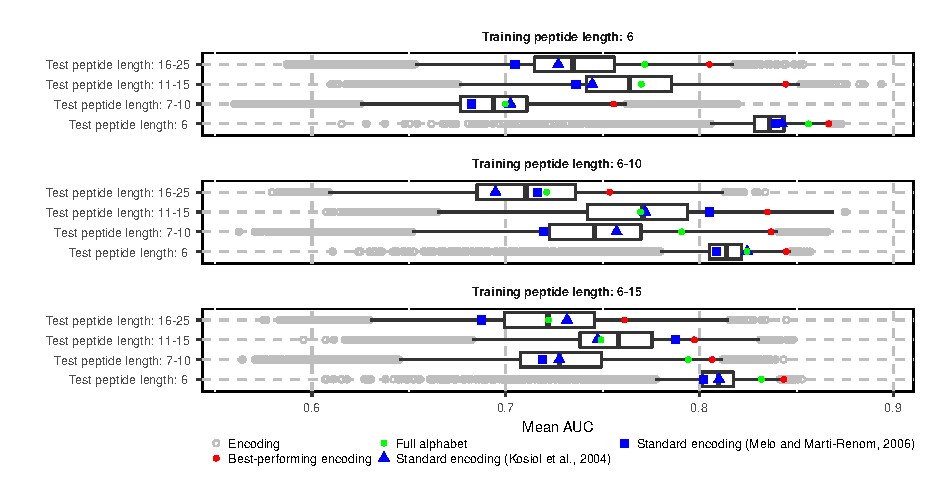
\includegraphics{figures/AUC_boxplot.eps}}
\caption{Distribution of mean AUC values of classifiers with various encodings 
for every possible combination of training and testing data set including 
different lengths of sequences. The left and right hinges of boxes correspond 
to 
the 0.25 and 0.75 quartiles. The bar inside the box represents the median. The 
gray circles correspond to the encodings with the AUC outside the 0.95 
confidence interval. 
}\label{fig:AUC_boxplot}

\end{figure*}

The predictor based on the best-performing encoding had the AUC always in the 
fourth quartile of all AUC values (Fig.~\ref{fig:AUC_boxplot}). It reached the 
highest AUC (0.8667) in classification of the shortest sequences (with the 
length of 6 residues) when the training set also consisted of the sequences of 
the same length. It results most probably from the pattern homogeneity of the 
short peptide set. 

  The most problematic was the correct prediction of the amyloidogenicity in the 
longest peptides, ranging from 16 to 25 residues, when the algorithm was trained 
also on longer peptides (6-10 and 6-15 data sets). Here the AUC value did not 
exceed 0.77. The weakest performance results from more complex organization of 
longer amylogenic peptides. In such peptides, only a very specific region of 
residues might be responsible for the creation of harmful aggregates. In this 
case, when overlapping hexamers are extracted, only part of them may carry the 
true signal of amyloidogenicity but all of them are marked as amyloids. 

  We also evaluated classifiers based on the full (i.e., unreduced) amino acid 
alphabet. In most cases, they were placed in the fourth quartile of the AUC 
values (Fig.~\ref{fig:AUC_boxplot}). Nevertheless, they never predicted 
amyloidogenicity better than the best classifier based on the reduced alphabet. 
It implies, that the amyloidogenicity can be described more accurately using less 
than 20 amino acids.

  Standard encodings included in the cross-validation has often AUC lower than 
the median. It implies that although the amyloidogenicity can be described by a 
reduced amino acid alphabet, such alphabet must consider only very special 
physicochemical properties of residues and cannot be too general.

\subsection{The best-performing encoding and important n-grams}


\begin{figure*}[h]
\centerline{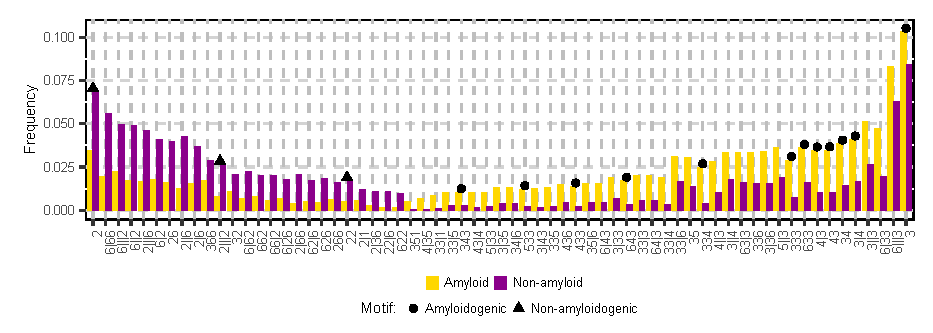
\includegraphics{figures/ngrams.eps}}
\caption{The frequency of important n-grams used by the best-performing 
classifier in amyloid and non-amyloid sequences. The elements of n-grams are 
amino acids encoded using the best-performing reduced amino acid alphabet. A 
vertical bar represents a gap in a n-gram between its elements. The frequency 
was computed using the total number of occurrences divided by the number of 
possible n-grams of their length. Dots and triangles denote n-grams occurring in 
motifs found in respectively amyloidogenic and non-amyloidogenic 
sequences~\citep{lopez_de_la_paz_sequence_2004}.}\label{fig:ngrams} 
\end{figure*}
% * <pamac@smorfland.uni.wroc.pl> 2016-05-26T23:01:59.166Z:
% Z czego ta czestosc? Kiedy sumuje sie do 100%? Moze to posortowac wg roznic w czestosciach miedzy dwoma grupami, albo wg czestosci amyloidow.
%
% ^.
% * <michalburdukiewicz@gmail.com> 2016-06-06T08:21:58.121Z:
%
% czestosc przeliczono na poszczegolne n-gramy i posortowano
%
% ^.

In total, eleven combinations of physicochemical properties created the best 
performing encoding. Only four features appeared in all combinations: 
hydrophobicity index~\citep{argos_structural_1982}, average flexibility 
indices~\citep{bhaskaran_positional_1988}, polarizability 
parameter~\citep{charton_structural_1982} and thermodynamic $\beta$-sheet 
propensity~\citep{kim_thermodynamic_1993}.

  The best encoding chosen in the analysis consists of six amino acid subgroups, 
which are characterized by distinct and specific properties: 1) G, 2) K, P, R, 
3) I, L, V, 4) F, W, Y, 5) A, C, H, M, 6) D, E, N, Q, S, T. The 3rd subgroup contains strongly hydrophobic amino 
acids. In the 4th subgroup, the amino acids show also aromatic properties. On 
the other hand, the most hydrophilic amino acids are in the 2nd and 6th 
subgroups . The former includes two strongly basic amino acids, whereas the latter 
% * <kotulska@gmail.com> 2016-06-12T14:25:26.706Z:
%
% > clearly
%
% clear-ly? Czy chodziło o coś innego?
%
% ^ <michalburdukiewicz@gmail.com> 2016-06-12T19:27:55.960Z:
%
% zmieniona na strongly
%
% ^.
two acidic and four polar residues. The first subgroup includes only glycine, 
which is the smallest amino acid and the most flexible.  By average, quite 
flexible amino acids are also present in the second subgroup, whereas the least 
flexible amino acids are in the subgroup 4 and 5. The glycine has also the 
lowest propensity to form $\beta$-sheet and the subgroups 3 and 4 largest. 

  We found 65 n-grams that had  obtained p-values smaller than 0.05 in QuiPT test 
% * <kotulska@gmail.com> 2016-06-12T14:28:05.679Z:
%
% >  We selected
%
% do czego? To biuld the final classifier ?
%
% ^ <michalburdukiewicz@gmail.com> 2016-06-12T19:29:47.246Z:
%
% nie, nie wybieralismy ich do ostatecznego klasyfikatora. To tylko obserwacja z analizy cross-validation
%
% ^.
in all repetitions of cross-validation, regardless of the lengths of sequences in 
the training set (see Fig.~\ref{fig:ngrams}). The frequency of the n-grams was 
computed for all sequences derived from AmyLoad . The n-grams typical of 
amyloidogenic sequences (with the highest frequency occurrence in amyloids) mostly  include 
highly hydrophobic amino acids with tendency to form $\beta$-structures, 
from subgroups 3 and 4. The n-grams occurring frequently in amyloids have often 
repeats of amino acids from the subgroup 3, suggesting that the presence of 
these amino acids in the vicinity might be one of the most effective predictors of 
amyloidogenicity.

  On the other hand, n-grams typical of non-amyloidogenic peptides have mostly 
amino acids belonging to subgroups 2 and 6. These subgroups include strongly 
hydrophilic and highly flexible amino acids (K, P, R, D, E), which hamper the 
formation of $\beta$-structures.

  Out of 65 the most informative n-grams, 15 (23\%) were also found in the motifs 
validated experimentally for amyloidogenic and non-amyloidogenic 
peptides~\citep{lopez_de_la_paz_sequence_2004}. The peptides used in this study are 
included in the AmyLoad data base, thus n-gram analysis is at least 
partially able to find the patterns in validated sequences.

\subsection{Benchmark of AmyloGram}

% latex table generated in R 3.2.3 by xtable 1.8-2 package
% Tue Mar  8 14:17:55 2016
\begin{table}[ht]
\centering
\small
\caption{Results of benchmark on \textit{pep424} data set for PASTA2, 
FoldAmyloid, AmyloGram and its version learned on n-grams extracted for full amino acid alphabet from the sequences of the lengths specified in 
the brackets.} 
\label{tab:bench_summary}
\begin{tabular}{ccccc}
  \toprule
Classifier & AUC & MCC & Sensitivity & Specificity \\ 
  \midrule
AmyloGram (6) & 0.8856 & 0.6057 & 0.6779 & 0.9037 \\
\rowcolor[gray]{0.85}AmyloGram (6-10) & \textbf{0.8972} & \textbf{0.6307} & 
0.8658 & 0.7889 \\ 
AmyloGram (6-15) & 0.8728 & 0.5420 & \textbf{0.9463} & 0.6111 \\ 
   \rowcolor[gray]{0.85}full alphabet (6) & 0.8411 & 0.5427 & 0.4966 & 
\textbf{0.9593} \\ 
  full alphabet (6-10) & 0.8581 & 0.5698 & 0.7517 & 0.8259 \\ 
   \rowcolor[gray]{0.85}full alphabet (6-15) & 0.8610 & 0.5490 & 0.8188 & 
0.7519 \\ 
\hline \hline
  PASTA2 & 0.8550 & 0.4291 & 0.3826 & 0.9519 \\ 
   \rowcolor[gray]{0.85}FoldAmyloid & 0.7351 & 0.4526 & 0.7517 & 0.7185 \\ 
  APPNN & 0.8343 & 0.5823 & 0.8859 & 0.7222 \\ 
   \bottomrule
\end{tabular}
\end{table}

The benchmark covered AmyloGram as well as the three peer-reviewed predictors of 
amyloidogenicity: physical models included in PASTA2~\citep{walsh_pasta_2014} and 
FoldAmyloid~\citep{garbuzynskiy_foldamyloid:_2010} as well as based on neural networks 
APPNN~\citep{familia_prediction_2015}. None of this methods is using 
reduced amino acid alphabet, but APPNN codes amino acids using the exact 
values of their physicochemical properties. Some known classifiers were 
not included in the benchmark because their performance on \textit{pep424} 
data set is already known and lower than the performance of PASTA2 and 
FoldAmyloid~\citep{walsh_pasta_2014}.

  We analyzed AUC, Matthew's Correlation Coefficient 
% * <kotulska@gmail.com> 2016-06-12T14:34:22.619Z:
%
% >  Under the Curve (AUC
%
% usunąłem rozwinięcie skrotu, wprowadzamy je wczesniej
%
% ^.
(MCC), sensitivity and specificity (see Tab.~\ref{tab:bench_summary}). We used 
default settings for FoldAmyloid and APPNN. PASTA2 evaluated the input data in the 
'Peptides' mode, which is adviced by its authors for a peptide data.

  Since PASTA2 does not return a probability of belonging to a specific category, 
we normalized the output data to compute the AUC values. The advised energy 
threshold (-5) was also normalized in the same manner and used as cut-off in 
computations of specificity, sensitivity and MCC. The resulting value of 
specificity 0.9519 is close to the value provided by its authors (0.95) and assures 
correctness of our computations. For other classifiers, including AmyloGram, we assumed a 
default 0.5 cut-off.
    
  In the case of the studied data set, the n-gram extraction method appeared 
efficient enough to produce classifiers able to outperform other published 
methods. AmyloGram showed the highest AUC and MCC among all tested classifiers 
and outperformed its counterparts trained using full amino acid alphabet. It 
is important to highlight that AmyloGram is the most balanced tool among all analyzed 
classifiers, having the best specificity/sensitivity trade-off, as indicated by 
the value of MCC.
 
  The specificity of AmyloGram is lower than the specificity of PASTA2 but it is 
a consequence of the usage of the threshold value optimized for 0.95 specificity 
for the latter. If we assume for the AmyloGram the same threshold for the 
specificity, our classifier will still have a higher sensitivity (0.5518) than 
PASTA2. Therefore, if we assume such thresholds to both predictors, they will detect true 
non-amyloids with the same specificity but AmyloGram will predict more true amyloids. 

  Two of  the three classifiers trained on  n-grams using  the full alphabet 
% * <kotulska@gmail.com> 2016-06-12T14:39:09.886Z:
%
% > n-gram
%
% the best? Jaki?
%
% ^ <michalburdukiewicz@gmail.com> 2016-06-12T19:36:40.517Z:
%
% uscislilem
%
% ^.
had also AUCs higher than PASTA2 and all three were more successful than 
FoldAmyloid as well as APPNN. They also maintained the high specificity as seen 
previously during cross-validation. However, they generally performed worse than 
the classifier based on the reduced amino acid alphabet.
  
  Among all considered predictors of amyloidogenicity, APPNN had the highest 
sensitivity. Nevertheless, its AUC was worse than AUCs of all n-gram-based 
predictors, as well as PASTA2  - indicating lower overall performance.

%  AmyloGram is trained to predict amyloidogenic, not amyloidic regions. Hence, 
%we did not test it on \textit{reg33} data set, which is commonly used to 
%evaluate the amyloid propensity of the full peptide 
%~\citep{tsolis_consensus_2013}.

\section{Conclusion}

The description of peptides by short sub-sequences (n-grams) followed by the 
reduction of the amino acid alphabet allowed us to create the efficient 
predictor of amyloidogenic sequences called AmyloGram. One of the strengths of 
this approach is its highly interpretable outcome, because our methods provide 
explicitly short motifs relevant to amyloidogenicity of peptides and 
discriminating amyloids from  non-amyloids. 65 important n-grams revealed that 
mostly alifatic and nonpolar amino acids (isoleucine, leucine and valine), 
together with aromatic and also hydrophobic amino acids (phenylalanine, 
tyrosine, tryptophan), are good predictors of amyloid peptides.

Polar and hydrophylic residues from group 2 (K, P, R) never occur in n-grams 
associated with amyloidogenicity which is confirmed also by the experimental 
studies. On the contrary, residues from group 6 (D, E, N, Q, S, T), also polar, 
are present in both in amyloidogenic and non-amyloidogenic sequences. It seems 
plausible, that amino acids belonging to group 6 are necessary for the proper 
formation of hot spot, but must be completed by hydrophobic residues from group 
3 or 4. That means that hot spots are not completely hydrophobic and should 
contain a fraction of hydrophilic residues with the exclusion for known 
breakers of $\beta$-structures as lysine, proline and arginine.

Our studies confirm that the most important physicochemical properties associated 
with amyloidogenicity are hydrophobicity and tendency to forming $\beta$-sheets.  
We additionally discovered that amino acid flexibility can also sufficiently 
discriminate amyloid and non-amyloid peptides. The aggregating peptides tend to
be characterized by more rigid chains.

Our findings can be helpful in understanding the process of amyloid aggregation 
and recognition of peptides susceptible to the formation of amyloid aggregates involved 
in various diseases. Moreover, they might be employed in the creation of synthetic 
amyloid peptides. We anticipate that the described workflow is versatile enough to 
be applied in other areas of protein function prediction.


\section*{Funding and availability}

Computations were carried out in Wroclaw Center for Networking 
and Supercomputing (\url{http://www.wcss.pl}) and funded by the
institutional grant No. 347. This research was partially funded by the KNOW Consortium and
National Science Center (2015/17/N/NZ2/01845).

Our software is accessible as the web server under address 
\url{www.smorfland.uni.wroc.pl/amylogram/}. The web tool constists of AmyloGram 
(6-10). The threshold can be manually specified by an user.

The code and results are publicly available at: \url{github.com/michbur/prediction_amyloidogenicity_ngram}.

\bibliography{amyloids}
\end{document}
